\documentclass[12pt]{article}
\usepackage[a4paper, margin=12mm]{geometry}
\usepackage{datatool}
\usepackage{graphicx}
\usepackage{ragged2e}
\usepackage{setspace}
\usepackage{xcolor}
\usepackage{fontawesome}
\usepackage{tabularx}
\usepackage[none]{hyphenat}
%\usepackage{showframe}

		\DTLloaddb{database}{data.csv}
\begin{document}  

		\DTLforeach{database}{
			\Sno=Sno, \Name=Name, \Institution=Institution, \Rs=Rs, \RsW=RsW}
		{
			

	\begin{center}
		\thispagestyle{empty}	
		\onehalfspacing
		{\large National Institute of Technology Puducherry, Karaikal}\\
		{An Institution of National Importance}\\ \vspace{-0.25cm}
		{under the Ministry of Education, Government of India}\\
		{\large  Thiruvettakudy, Karaikal, Union Territory of Puducherry 609 609, India}
	\end{center}
		
	\begin{center}
		{\large $2^{nd}$ National Conference on Communication Systems (NCOCS-2020)}\\
		November 21, 2020\\
		\vspace{0.15cm}
		{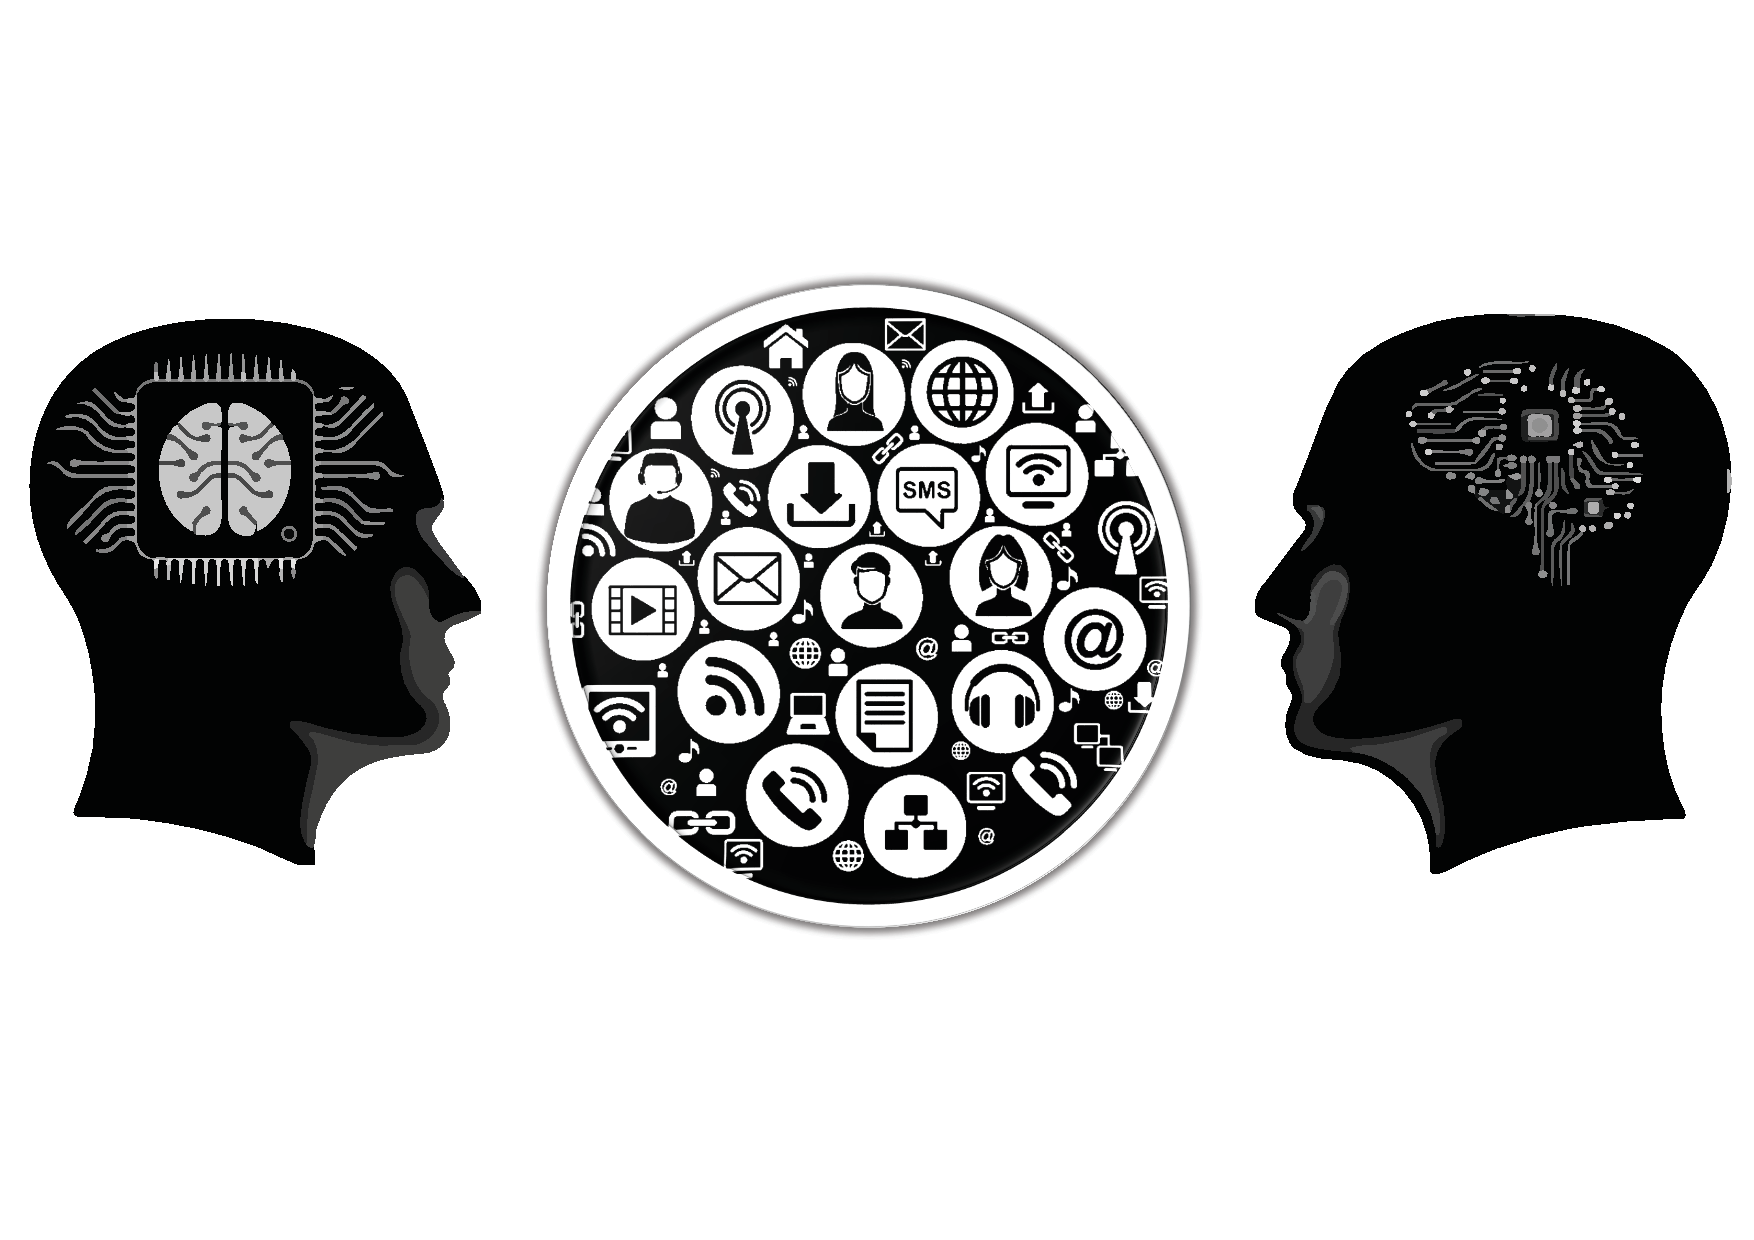
\includegraphics[scale=0.16,trim={0cm, 4.5cm, 0cm, 4cm},clip]{conference-logo.pdf}}\\
		\textit{Signal Processing and Machine Learning Techniques for Communication}\\
		\vspace{0.25cm}
		{Organized by}\\
		\vspace{0.15cm}
		\includegraphics[scale=0.12]{nitpy-logo.png}\\ \vspace{0.25cm}
		Department of Electronics and Communication Engineering\\
		National Institute of Technology Puducherry, Karaikal \\
		\vspace{0.25cm}
		In association with\\ \vspace{0.25cm}
		\begin{table}[h!]
			\centering
			\small
			\begin{tabular}{cc}
				\multicolumn{1}{c}{\includegraphics[scale=0.20]{ISTE-logo.pdf}} & \multicolumn{1}{c}{\includegraphics[scale=0.20]{IEI-logo.pdf}} \\ 
				\begin{tabular}[c]{@{}c@{}}{Indian Society for Technical Education}\\
					{Under the Societies Registration Act XXI of 1860}\\
					{New Delhi}\end{tabular} & 
				\begin{tabular}[c]{@{}c@{}}{The Institution of Engineers (India)} \\
					{Established 1920, Incorporated by Royal Charter 1935}\\
					{Puducherry State Centre, Puducherry}
				\end{tabular}                       \\ 
			\end{tabular}
		\end{table}
			
	\underline{RECEIPT}\\ 
		\vspace{0.5cm}
		\justifying 
		\onehalfspacing
%		\noindent Received with thanks from \textbf{\Name}, {\Institution}, an amount of \faInr~\Rs/- (\RsW)~as registration fees for the $2^{nd}$ National Conference on Communication Systems (NCOCS-2020), organized by the Department of Electronics and Communication Engineering, National Institute of Technology Puducherry, Karaikal, India, on November 21, 2020.
		\begin{tabularx}{0.94\linewidth}{ l X }
			& 
			\justifying 
			\onehalfspacing
			{\noindent Received with thanks from \textbf{\Name}, {\Institution}, an amount of \faInr~\Rs/- (\RsW)~as registration fees for the $2^{nd}$ National Conference on Communication Systems (NCOCS-2020), organized by the Department of Electronics and Communication Engineering, National Institute of Technology Puducherry, Karaikal, India, on November 21, 2020.}
			\\
		\end{tabularx}
	\end{center}
	
	\vspace{0.25cm}
	\raggedright \underline{Receipt No.:~\#\Sno}
	
	\vspace{2cm}
	\begin{flushright}
		Dr. G. Lakshmi Sutha                 \\
		Chairperson (NCOCS-2020),             \\
		Assistant Professor \& Head (ECE),   \\
		NITPy, Karaikal, India.                           
	\end{flushright}
	

	\newpage
}

\end{document}